\documentclass[../main/main.tex]{subfiles}
\begin{document}



\chapter{Perturbation Theory}

In this chapter we will discuss perturbation theory using path integral approach. Also, we will see that path integrals contains more information than perturbation theory, since path integrals allows to study non-perturbative features, that are not involved in the  perturbative approach. We will see that perturbative expansion has a limited fidelity to physics feature we want to analyze, even at highest order of expansion. 

\section{Correlators and scattering amplitudes}

\textsf{Skinner~\cite{Skinner:2018aa} sec. 1.2.2, 1.2.4}\\

Primary object we will use to describe perturbative approach to QFT are the partition functions
\[\mathcal Z(g,m,\lambda,\dots)=\int_C\mathcal D\phi \,e^{\frac i\hbar S[\phi]}\]
As we already mentioned, the partition function does not depend directly from fields , but only on the other parameters of the theory. Using partition functions, we want to compute correlation functions, which are genericay expectation values of products of operators of these fields
\begin{equation}\label{eqn:exp-value-prod-corr}\boxed{
\left\langle\prod_{i=1}^nO_i(\phi)\right\rangle=\frac1{\mathcal Z}\int_C\mathcal D\phi \,e^{\frac i\hbar S[\phi]}\prod_{i=1}^nO_i(\phi)
}\end{equation}
Here we introduced the normalization factor $1/\mathcal Z$ so that the expectation value of operator 1 is unitary: $\langle1\rangle=1$. We introduced this normalizations since we want to use correlation functions to compute scattering amplitude using LSZ formula. 

Usually operators $O_i(\phi)$ are \emph{local operators}, this means that they depend on the value of $\phi$ and/or its derivatives at a point of the spacetime $p\in M$. Some example of local operators may be $\phi^4(x)$, $\phi(x)\partial_\mu\phi(x)\partial^\mu\phi(x)$, etc. Other important operators are \emph{integrated operators} over the full space time, for instance $\int_M\de^4x(\partial_\mu\phi\partial^\mu\phi)^2$. We can also integrate over some submanifold of $M$, for example this is what we do for \emph{Wilson lines}, which is a fundamental object in gauge theories defined in terms of a given connections $A$ on the gauge field and a certain closed path $\Gamma$
\vspace{-0.5cm}
\[\mathcal W_\Gamma=\Tr(-\oint_\Gamma\de x^\mu A_\mu)
\qquad\quad
\raisebox{-1cm}{
\begin{tikzpicture}[x=0.75pt,y=0.75pt,yscale=-1,xscale=1]
\draw    (239.3,173.79) .. controls (232.75,151.54) and (249.05,112.33) .. (265.88,134.64) .. controls (282.38,155.95) and (316.29,158.19) .. (294.59,173.84) .. controls (285.8,178.31) and (255.18,176.47) .. (269.03,189.74) .. controls (284.07,205.31) and (248.5,201.19) .. (240.1,176.56) ;
\draw [shift={(239.3,173.79)}, rotate = 436.39] [fill={rgb, 255:red, 0; green, 0; blue, 0 }  ][line width=0.08]  [draw opacity=0] (8.93,-4.29) -- (0,0) -- (8.93,4.29) -- cycle    ;
\draw (221.56,172.66) node    {$\Gamma $};
\end{tikzpicture}
}\]
All these operators can be computed directly using correlation functions. 

One important point in the following, is that operators can be directly related to partition functions. Imagine for instance an action $S[\phi]$ that is given by
\[S[\phi]=\int_M\de^4x\left[-\frac12\partial_\mu\phi\partial^\mu\phi+\frac\lambda{4!}\phi^4(x)\right]\]
Now we see that if we want to compute the expectation value of the operator $O$ defined as
\[\langle O\rangle=\left\langle\frac1{4!}\int_M\de^4x\,\phi^4(x)\right\rangle\]
then it can be written in terms of the partition function
\begin{align*}
\left\langle\frac1{4!}\int_M\phi^4(x)\de^4x\right\rangle
&=\int_C\mathcal D\phi\p{\frac{1}{4!}\int\de^4x\phi^4(x)}\,e^{\frac i\hbar S[\phi]}
=-i\hbar\frac{\partial}{\partial\lambda}\int_C\mathcal D\phi \,e^{\frac i\hbar S[\phi]}
=-i\hbar\frac{\partial}{\partial\lambda}\mathcal Z
\end{align*}
Now, suppose that in my initial theory the action contains only the integral of $-\frac12\partial_\mu\phi\partial^\mu\phi$ and we want to study the response of the theory when we add the additional term $\frac\lambda{4!}\phi^4(x)$ to the integrand of the action. Such a response is meant to be exactly the expectation value we just calculated. 
This implies that I can measure the response of the theory to the additional local operator by varying the partition function with respect to the coupling $\lambda$. 

Let's generalize what we already stated. Image that I have an initial theory with action $S[\phi]$ (for example $S[\phi]=\int_M\de^4x\,\p{-\frac12\partial_\mu\phi\partial^\mu\phi}$) and I introduce a coupling term $\int_M\de^4xJ(x)O(x)$ as a perturbation to my initial theory. The function $J(x)$ is a called \emph{local coupling}, or more traditionally ``\emph{source}'', and generalize the parameter $\lambda$, while $O(x)$ is an operator (for instance $O(x)=\frac1{4!}\phi^4(x)$). I can measure the response of my QFT to the addition of the operator $O$ by doing the following substitution
\begin{equation}\boxed{
S[\phi]\quad\to\quad S[\phi]+\int_M\de^4xJ(x)O(x)
}\end{equation}
and then taking derivatives of the partition function:\footnote{We introduce normalization $1/\mathcal Z$ in order to normalize probabilities and we omit the time ordering product in the expectation value.}
\begin{equation}\label{eqn:exp-value-prod-deriv}\boxed{
\langle O_1(x_1)O_2(x_2)\dots O_n(x_n)\rangle=\frac{(-i\hbar)^n}{\mathcal Z}\frac{\delta^n\mathcal Z[J_i]}{\delta J_1(x_1)\delta J_2(x_2)\dots \delta J_n(x_n)}\bigg\vert_{J_i=0}
}\end{equation}
Notice that taking $J_i=0$ at the end of the computation we removed the additional factor $\int_M\de^4xJ(x)O(x)$ we added before in the action. 
This is a generic way to obtain the value for the expectation value of products of operators using functional derivatives instead of direct computation. For instance
\[\langle\phi(x_1)\phi(x_2)\dots\phi(x_n)\rangle=\frac{(-i\hbar)^n}{\mathcal Z}\frac{\delta^n\mathcal Z[J]}{\delta J(x_1)\delta J(x_2)\dots \delta J(x_n)}\bigg\vert_{J=0}\]
where we made the substitution
$S\to S+\int\de^4x \,J(x)\phi(x)$.
Actually we can have even more complicated operators such as stress energy tensor of the general relativity. 

Let's summarize our result: once we have our path integral and we defined our partition functions we can compute expectation values by using both eq.~\eqref{eqn:exp-value-prod-corr} and eq.~\eqref{eqn:exp-value-prod-deriv}, i.e. respectively either introducing operators in the partition function or introducing a local coupling in the action by mean of some function $J(x)$ and then taking variation with respects to this source.  

This allows us to split our problem in a free theory for which we will be able to compute path integral explicitly, and some additional operators (that also may describe interactions) for which we can compute the contributions to our theory using perturbative approach by taking variations of the partition function with respect to the sources that couple to these operators. 

In the special case of scattering amplitudes, we can obtain more specific forms for the previous results. Let's prescribe some asymptotic configuration for $\phi$, namely $\phi_i$ for $t\to-\infty$ and $\phi_f$ for $t\to+\infty$. Then the scattering amplitude is
\[\braket{\phi_f}{\phi_i}=\int_{C[\phi_f,\phi_i]}\mathcal D\phi\,e^{\frac i\hbar S[\phi]}\]
In order to compute scattering amplitudes we will use correlators through the LSZ formula, and we will compute correlators by splitting the action in the quadratic part for which we can compute correlators in an exact way and additional contributions which are going to be treated perturbatively. 


\section{Free field theory}

\textsf{Skinner~\cite{Skinner:2018aa} sec. 2.1, 2.2; Vafa~\cite{Hori:2003ic} 9.0, 9.1}\\

Let's start from the free field theory. We start from the special case of QFT in zero dimensions. This means that the manifold of out theory is just a point $M=\{p\}$ (we assume $M$ to be connected) and therefore there are no derivatives, we just have functions from a point to some target space (eg. $\RR$, $\CC$, etc.). Moreover, the space does not have any symmetry (for example, in such a theory spin doesn't exists). We can take fields as functions
\[\phi:\{p\}\longrightarrow\RR\]
In this case the partition function is just the Lebesgue integral (we can consider it in the Euclidean form)
\[\mathcal Z=\int_\RR\de\phi\,e^{-\frac{S[\phi]}\hbar}\]
were we used $-1$ instead of $i$ because since we are computing a Lebesgue integral we hope that the minus factor will give to the integral a generic good behaviour (notice that for most theories kinetic terms have positive contributions to the action). Also we assume for simplicity that $S[\phi]$ is polinomial, in particular we consider the quadratic case. 
Then in this case the theory is characterized by an action
\[S=\frac12M_{ij}\phi^i\phi^j\qquad\quad i,j=1,\dots,n\]
For simplify further the computation we take the matrix $M_{ij}$ to be a real, symmetric, positive defined matrix (in this way this matrix has only real positive eigenvalues).
The partition function for such a simple instance is 
\begin{equation}\label{eqn:part-func-free-0D}
\mathcal Z_0=\int_{\RR^n}\de^n\phi \exp{-\frac1{2\hbar}M_{ij}\phi^i\phi^j}=\frac{(2\pi\hbar)^{n/2}}{\sqrt{\det M}}
\end{equation}
where we can computed easily the integral by diagonalization of the matrix $M$ through orthogonal rotations $O(n)$. Since the Lebesgue measure is invariant under orthogonal rotations, we just have to compute the $n$-dimensional Gaussian integral we obtained in this way. 

In general using Gaussian integrals we will always be able to compute quadratic terms. Hence we will call ``free fields'' theories which contains only quadratic terms of my action. In the perturbative approach possibly I will expand my action and I will do this in such a way that the first term that appears up to constant pieces is going to be a quadratic term in the field, and that is going to be the free theory. 

\subsubsection{Correlators in the free theory}

Now we take into account correlators in the free theory:
\[\langle\phi^{a_1}\dots\phi^{a_n}\rangle=\frac1{\mathcal Z_0}\int_{\RR^n}\de^n\phi\,\,\phi^{a_1}\dots\phi^{a_n}\exp{-\frac1{2\hbar}M_{ij}\phi^i\phi^j}\]
We will compute this by means of introduction of sources:
\begin{align*}
\langle\phi^{a_1}\dots\phi^{a_n}\rangle
&=\frac1{\mathcal Z_0}\int_{\RR^n}\de^n\phi\,\phi^{a_1}\dots\phi^{a_n}\exp{-\frac1{2\hbar}M_{ij}\phi^i\phi^j-\frac{1}\hbar J_i\phi^i}\Bigg\vert_{J_i=0}\\
&=\frac1{\mathcal Z_0}\int_{\RR^n}\de^n\phi\,(-\hbar)^n\frac{\delta^n}{\delta J_{a_1}\dots \delta J_{a_n}}\exp{-\frac1{2\hbar}M_{ij}\phi^i\phi^j-\frac{1}\hbar J_i\phi^i}\Bigg\vert_{J_i=0}\\
&=\frac{(-\hbar)^n}{\mathcal Z_0}\frac{\delta^n}{\delta J_{a_1}\dots \delta J_{a_n}}\p{\int_{\RR^n}\de^n\phi\,\exp{-\frac1{2\hbar}M_{ij}\phi^i\phi^j-\frac{1}\hbar J_i\phi^i}}\Bigg\vert_{J_i=0}
\end{align*}
We just followed the procedure described in the previous section. Starting from the free theory we added the coupling with the source, then we took derivatives that brings down fields. Computing the partition function for the theory with sources we can immediately obtain the correlation function by means of derivatives. 

Now, we have in the exponential a term quadratic in fields and a term linear in fields. We can redefine fields in order to absorb the linear terms as follow:
\[\widetilde\phi^i=\phi^i+(M^{-1})^{ij}J_j\]
This is just a translation, therefore the measure does not change $\de^n\widetilde\phi=\de^n\phi$. The argument of the exponential become:
\begin{align*}
-\frac12M_{ij}\phi^i\phi^j-J_i\phi^i
&=-\frac12M_{ij}\p{\widetilde\phi^i-(M^{-1})^{ik}J_k}\p{\widetilde\phi^j-(M^{-1})^{jl}J_l}-J_i\p{\widetilde\phi^i-(M^{-1})^{ik}J_k}\\
&=-\frac12M_{ij}\widetilde\phi^i\widetilde\phi^j+\frac12J_i(M^{-1})^{ij}J_j
\end{align*}
Then I can complete the calculation of the correlator
\begin{align*}
\langle\phi^{a_1}\dots\phi^{a_n}\rangle
&=\frac{(-\hbar)^n}{\mathcal Z_0}\frac{\delta^n}{\delta J_{a_1}\dots \delta J_{a_n}}\p{\int_{\RR^n}\de^n\phi\,\exp{-\frac1{2\hbar}M_{ij}\widetilde\phi^i\widetilde\phi^j+\frac1{2\hbar}J_i(M^{-1})^{ij}J_j}}\Bigg\vert_{J_i=0}
\end{align*}
and since the first term in the exponential cancel with normalization factor $\mathcal Z_0$ we finally end up with
\begin{equation}\label{eqn:0-dim-corr-fin}\boxed{
\langle\phi^{a_1}\dots\phi^{a_n}\rangle
=(-\hbar)^n\frac{\delta^n}{\delta J_{a_1}\dots \delta J_{a_n}}\exp{\frac1{2\hbar}J_i(M^{-1})^{ij}J_j}\Bigg\vert_{J_i=0}
}\end{equation}

From this expression I learn that
\begin{enumerate}[label=\textbullet]
\item The number of derivatives that I have to take must be even, otherwise all this expression vanishes when I take $J_i=0$, therefore each correlator of an odd number of operator gets zero as result;
\item For $n=2$ the correlator corresponds to the \emph{propagator}
\begin{align*}
\langle\phi^a\phi^b\rangle
&=\hbar^2\frac{\delta^2}{\delta J_{a}\delta J_{b}}\exp{\frac1{2\hbar}J_i(M^{-1})^{ij}J_j}\Bigg\vert_{J_i=0}\\
&=\hbar\frac{\delta}{\delta J_{b}}\p{(M^{-1})^{aj}J_j\exp{\frac1{2\hbar}J_i(M^{-1})^{ij}J_j}}\Bigg\vert_{J_i=0}
=\hbar(M^{-1})^{ab}
\end{align*}
I could have expected this feature since in zero dimensional theories propagators are just the inverse of quadratic forms. This will be different in higher dimensions since in that case propagators will be inverse of differential operators of the second order. 

Associated to each correlator there is a Feynman diagram, which in zero dimension is very simple
\begin{equation}\label{eqn:contraction-2fields-0dim}
\langle\phi^a\phi^b\rangle=\quad\phi^a\,
\raisebox{0.5mm}{\begin{tikzpicture}
	\begin{feynman}
		\vertex(a);
		\vertex[right=1.5cm of a](b);
		\diagram*{(a)--(b)};
	\end{feynman}
\end{tikzpicture}}\,\,
\phi^b\quad= \hbar(M^{-1})^{ab}
\end{equation}
\item Contributions of the initial partition function $\mathcal Z_0$ are normalized to 1, this implies that we don't have to calculate explicitly the partition function and our procedure is defined even if $\mathcal Z_0$ is divergent. Everything ends up to an easy computation given by the simple term eq.~\eqref{eqn:0-dim-corr-fin} that depends only on the sources. 
\end{enumerate}

\subsubsection{Wick's theorem}
In the general case, when we want to compute the correlator between $2k$ fields we have to sum over products of all inequivalent ways of connecting pairs of $\phi^i$ using $M^{-1}$:
\begin{equation}\label{eqn:wick-thm}
\langle\phi^{a_1}\dots\phi^{a_{2k}}\rangle=\hbar^k\sum_{\sigma\in\text{Pairings}}\,\,\,\prod_{i\in\sigma_{\text{Pairs}}}(M^{-1})^{i\sigma(i)}
\end{equation}
This is just the statement of the \emph{Wick's theorem}. For instance
\begin{equation}\label{eqn:wick-thm-case4}
\langle\phi^a\phi^b\phi^c\phi^d\rangle=\hbar^2\left[(M^{-1})^{ab}(M^{-1})^{cd}+(M^{-1})^{ac}(M^{-1})^{bd}+(M^{-1})^{ad}(M^{-1})^{bc}\right]
\end{equation}
Formula eq.~\eqref{eqn:wick-thm} comes from eq.~\eqref{eqn:0-dim-corr-fin}: in order to have non vanishing terms, couples of derivatives must acts in such a way they brings down matrix elements $(M^{-1})^{ab}$ independent from sources. In other words eq.~\eqref{eqn:wick-thm} states that contributions to $\langle\phi^{a_1}\dots\phi^{a_{2k}}\rangle$ are given by all possible products of contractions, and each contraction gives a factor $\hbar(M^{-1})^{ab}$, as shown in \eqref{eqn:contraction-2fields-0dim}. For example, correlator eq.~\eqref{eqn:wick-thm-case4} is given by following pairings
\[
\begin{tikzpicture}[baseline=(e)]
	\begin{feynman}
		\vertex(e);
		\vertex[above left=0.5cm of e](a){$1$};
		\vertex[below left=0.5cm of e](b){$2$};
		\vertex[above right=0.5cm of e](c){3};
		\vertex[below right=0.5cm of e](d){4};
		\diagram*{(a)--(b), (c)--(d)};
	\end{feynman}
\end{tikzpicture}
\quad+\quad
\begin{tikzpicture}[baseline=(e)]
	\begin{feynman}
		\vertex(e);
		\vertex[above left=0.5cm of e](a){$1$};
		\vertex[below left=0.5cm of e](b){$2$};
		\vertex[above right=0.5cm of e](c){3};
		\vertex[below right=0.5cm of e](d){4};
		\diagram*{(a)--(c), (b)--(d)};
	\end{feynman}
\end{tikzpicture}
\quad+\quad
\begin{tikzpicture}[baseline=(e)]
	\begin{feynman}
		\vertex(e);
		\vertex[above left=0.5cm of e](a){$1$};
		\vertex[below left=0.5cm of e](b){$2$};
		\vertex[above right=0.5cm of e](c){3};
		\vertex[below right=0.5cm of e](d){4};
		\diagram*{(a)--(d), (c)--(b)};
	\end{feynman}
\end{tikzpicture}
\]
All possible contractions for $2k$ fields are\footnote{When I take the first field, I have $2k-1$ ways to couple it. Then I take one of the other $2k-2$ fields, and I have $2k-3$ way to couple this one, and so on.}
\begin{equation}\label{eqn:Wick-n-possible-contr}
(2k-1)(2k-3)\dots(1)=\frac{2k}{2k}(2k-1)\frac{(2k-2)}{2(k-1)}(2k-3)\dots1=\frac{(2k)!}{2^kk!}
\end{equation}
This is the number of all the Feynman diagrams I obtain through contractions when I do perturbation theory. 


\section{Perturbation theory}

\textsf{Skinner~\cite{Skinner:2018aa} sec. 2.3; Vafa~\cite{Hori:2003ic} 9.0, 9.1}\\

Now, we want to compute correlator functions or in general expectation values for operators (let's consider the simply case of one field $\phi$):
\begin{equation}\label{eqn:correlator-f-pert}
\langle f(\phi)\rangle=\frac1{\mathcal Z}\int_\RR\de\phi\, f(\phi)e^{-S[\phi]/\hbar}
\end{equation}
Even in this simple instance, where we are considering zero dimensions and the path integral is a standard integral, the exact computation is in general impossible, neither if we consider $f$  a simple function. For this reason is often very useful to use perturbation theory, indeed in many case it gives very good results. Usually when we consider perturbation theory we start from classical results and then we calculate quantum corrections. The general idea to do this is to take $\hbar\to0$ to obtain the classical result and then expand in powers of $o(\hbar)$

We will see that  the Taylor expansion in $\hbar$ that we will do is in general not well defined. Take for instance $\hbar>0$, then the series we obtain from eq.~\eqref{eqn:correlator-f-pert} may converge, but for $\hbar<0$ the series diverges for sure. We cannot assume simply $\hbar>0$, since in order to use the Taylor expansion, we need to have some neighbourhood of the origin where the expansion in well defined, and with the restriction $\hbar>0$ such neighbourhood have radius equal to 0.  

The best we can do is to introduce an \textbf{asymptotic expansion}, i.e. we introduce a series $\sum_{n=0}^\infty a_n\hbar^n$ such that for each \emph{finite} $N\in\mathbb N$ it approaches our function $F(\hbar)$:
\begin{equation}\label{eqn:asymp-expan-pert}
\lim_{\hbar\to0^+}\frac1{\hbar^N}\Bigg\vert F(\hbar)-\sum_{n=0}^Na_n\hbar^n\Bigg\vert=0
\qquad\forall N\in\mathbb N
\end{equation}
This means that for each $N$ fixed we can choose a sufficiently small value for $\hbar$ such that the difference between the initial function and our asymptotic expansion is $O(\hbar^N)$. Raising the value for $N$ we can obtain better reproductions of $F(\hbar)$, but notice that 
\begin{enumerate}[label=\textbullet]
\item what we stated right now holds if $\hbar\to0^+$, but this is not true  for fixed (even if very small) values of $\hbar$ , like in the physical case: an asymptotic expansion for finite values of $\hbar$ can't be obtained in general. Indeed, for fixed values of $\hbar$ we can use eq.~\eqref{eqn:asymp-expan-pert} only for finite values of $N$, since over some value of $N$ contributions in the order of $\hbar^N$ became relevant in our analysis;
\item even if we trust our asymptotic expansion, we lose in any case all transcendental terms, i.e. terms that are sums of exponentials. For instance $F(\hbar)$ and $\widetilde F(\hbar)=F(\hbar)+Ae^{-B/\hbar^2}$ have same asymptotic expansion for $\hbar\to0$, since $e^{-B/\hbar^2}\to0$ when we take the limit. Usually these terms are small and can be neglected, anyhow in general one may be interested in these contributions, that cannot be obtained through asymptotic expansion. 
\end{enumerate}
Notice that these additional informations were contained in the initial path integral eq.~\eqref{eqn:correlator-f-pert}, but are lost in the perturbative approach. As we already stated, path integral contains \emph{more} information than perturbation theory. 

\subsubsection{Perturbation theory for an interacting model}

Suppose we have an action $S[\phi]$ and we expand it around some minimum $\phi_0$  in a constant term plus a quadratic piece
\[S(\phi)=S(\phi_0)+\frac12\partial_\phi^2S(\phi_0)\delta\phi^2+\dots\]
The constant term is removed by the normalization into the partition function, then we can neglect it. We assumed that $\partial_\phi S(\phi)=0$ but even if this is not true we can obtain it by redefine our field removing any linear field. The quadratic part was already analyzed in the last section, since it describes a free theory at the vacuum $\phi_0$. Remaining terms are the one we will consider in our perturbative approach. 

What we essentially do is to split the action into 
\[S(\phi)=S_0(\phi)+S_I(\phi)\]
where $S_0(\phi)$ corresponds to the quadratic free theory and $S_I(\phi)$ is an interacting term. Let's start with a simple calculation of the expansion of the interacting part. Suppose that
\begin{equation}\label{eqn:action-examp-0d-perturb}
S(\phi)=\frac12m^2\phi^2+\frac\lambda{4!}\phi^4\quad,\quad S_0(\phi)=\frac12m^2\phi^2\quad\text{and}\quad S_I(\phi)=\frac\lambda{4!}\phi^4
\end{equation}
where $m^2>0$ and $\lambda>0$. In such a way $\phi=0$ is a global minimum, hence $S(\phi_0)=0$ and $\partial_\phi S=0$, and we have to expand around $\phi=0$, i.e. $\phi$ can be interpreted as a fluctuation around zero. Then the partition function of the free theory depends only on the mass
\[\mathcal Z_0(m^2)=\int_\RR\de\phi \exp{-\frac1{2\hbar}m^2\phi^2}\]
while the partition function depends also on the parameter $\lambda$:
\[\mathcal Z(m^2,\lambda)=\int_\RR\de\phi \exp{-\frac1{2\hbar}m^2\phi^2-\frac\lambda{4!\hbar}\phi^4}\]
We introduce the interaction as a response to the coupling with $\lambda$, using a source $J$
\begin{equation}\label{eqn:corr-exp-perturb-exp}
\mathcal Z(m^2,\lambda)=\int_\RR\de\phi \exp{-\frac1{2\hbar}m^2\phi^2-\frac\lambda{4!\hbar}\phi^4-\frac1\hbar J\phi}\Bigg\vert_{J=0}
\end{equation}
such that we recover the exponential of the interacting part as an operator inside the partition function of the free theory with the source:
\[\mathcal Z(m^2,\lambda)=\int_\RR\de\phi \,O(\phi)\exp{-\frac1{2\hbar}m^2\phi^2-\frac1\hbar J\phi}\Bigg\vert_{J=0}
\qquad\text{with}\qquad O(\phi)=\exp{-\frac\lambda{4!\hbar}\phi^4}\]
Then we see that the result of this integral is
\[\mathcal Z(m^2,\lambda)=\langle O(\phi)\rangle_0\,\mathcal Z_0(m^2)\]
Using the procedure we described before we have
\begin{align*}
\mathcal Z(m^2,\lambda)
&=\exp{-\frac\lambda{4!\hbar}\p{-\hbar\frac\partial{\partial J}}^4}\,\mathcal Z_0(m^2,J)\Bigg\vert_{J=0}\\
&=\sum_n\frac1{n!}\p{-\frac\lambda{4!\hbar}}^n\p{-\hbar\frac\partial{\partial J}}^{4n}\int_\RR\de\phi \,\exp{-\frac1{2\hbar}m^2\phi^2-\frac1\hbar J\phi}\Bigg\vert_{J=0}\\
&=\int_\RR\de\phi \,\exp{-\frac1{2\hbar}m^2\phi^2}\sum_n\frac1{n!}\p{-\frac\lambda{4!\hbar}}^n\phi^{4n}
\end{align*}
Even though eq.~\eqref{eqn:corr-exp-perturb-exp} could be computed directly using expansion in $\lambda$, this is not in general possible, while our procedure can be actually done also in more complex cases. In this simply case we can go on in the computation in an explicit way, in order to understand better the result we will obtain in general. If we set $\phi=\sqrt{2\hbar x/m^2}$ and $\de\phi=\sqrt{2\hbar/m^2}\,\de x/(2\sqrt x)$, and we change sign of the field for $\phi\in(-\infty,0)$ (this gives us an additional factor 2 which cancel the factor 1/2 in the Jacobian of the change of variable), we obtain
\begin{align*}
\mathcal Z(m^2,\lambda)
&=\sqrt{\frac{2\hbar }{m^2}}\int_0^{+\infty}\de x\,\frac{e^{-x}}{\sqrt x}\sum_n\frac1{n!}\p{-\frac{\lambda}{4!\hbar}}^n\p{\frac{2\hbar}{m^2}}^{2n}x^{2n}\\
&=\frac{\sqrt{2\hbar}}m\sum_n\frac1{n!}\p{-\frac{\lambda\hbar}{3!m^4}}^n\underbrace{\int_0^{+\infty}\de x\,x^{2n+\frac12-1}e^{-x}}_{\Gamma\p{2n+\frac12}}\\
&=\underbrace{\frac1m\sqrt{2\pi\hbar}}_{\mathcal Z_0(m^2)}\sum_n\p{-\frac{\lambda\hbar}{m^4}}^n\frac1{(4!)^nn!}\frac{(4n)!}{4^n(2n)!}\\
&=\mathcal Z_0(m^2)\p{1-\frac{\lambda\hbar}{m^4}\frac{4!}{4!\,1!\,4\,2!}+\dots}
\end{align*}
where we used the Gamma function
\begin{equation}\label{eqn:Gamma-function}
\Gamma(z)=\int_0^{+\infty}e^{-x}x^{z-1}\de x
\end{equation}
with proprieties
\[\Gamma(p)=p!\qquad\quad\Gamma\p{p+\frac12}=\sqrt\pi\,\frac{(2p)!}{4^pp!}\]
and equation eq.~\eqref{eqn:part-func-free-0D}. The final result in the last step shows explicitly the perturbative contributions to the partition function. 

We stress the fact that our result is not a Taylor expansion of the initial partition function, but is just an asymptotic expansion, as we stated in the beginning of this section. This is because, in our calculation, we were not really allowed to interchange the integral with the summation over $n$. 

Notice also that the expansion is actually in terms of $(\lambda\hbar)^n$ and not only in terms of $\lambda^n$. This is because each correction in $\lambda$ corresponds to a quantum correction, i.e. takes a factor $\hbar$. Moreover, we could have expected the factor $(-\lambda\hbar/m^4)^n$ simply by dimensional analysis, because the action has dimension $\hbar$, therefore by eq.~\eqref{eqn:action-examp-0d-perturb} follows that $\lambda$ and $m^2$ has both dimension $\hbar$.

Moreover, the term $1/((4!)^nn!)$ is fixed by the order of the expansion of the exponential. The other term $(4n)!/(4^n(2n)!)$ is going to be the number of ways we can join the $4^n$ fields given by each term of the expansion of my correlator, as described by eq.~\eqref{eqn:Wick-n-possible-contr} (we have to replace $k=2n$). 

Finally, notice that the result we obtain diverges. This is not a problem since we computed an asymptotic expansion, which not recovers the real initial partition function (anyhow, in general also the initial partition function may diverges, in this case we have to treat fields in correlators in such a way that divergent partition function is normalized at the end of the calculation). Recall Stirling approximation $n!\approx\exp{n\log n}$, this means that $(4n)!/((4!)^nn!)(4^n(2n)!)$ behaves like $\exp{n\log n+\dots}$ and this function has zero convergence radius. This number will corresponds to the number of Feynman diagrams one obtain at each perturbative level, and this means that above some order the number of Feynman diagrams that contributes is so huge that overcomes the small pre-factor $(-\hbar\lambda/m^4)^n$ and gives divergent contribution to the full series. Hence,  using perturbative approach to compute scattering amplitudes, up to some value $N$ the introduction of higher order contributions gives more precise results, but beyond that value my scattering amplitude will start to diverge. Obviously this behaviour of the series leads to some doubt about the using of perturbative expansion but this is, again, a consequence of the use of asymptotic expansion instead of Taylor's one. Moreover, sometimes non-perturbative effects, allows series to converges, as we will see later on. Anyhow,  these divergent contributions appears when we consider perturbative contributions many orders of magnitude away from the highest precision we will ever be able to archive experimentally. This means that asymptotic expansion have issues only from the mathematical point of view, while our results agree perfectly with physical results, and we are always be able to understand when our approach starts to show unphysical results. 


\subsection{Feynman Diagrams}

\textsf{Skinner~\cite{Skinner:2018aa} sec. 2.3.1}\\

Now we want to express perturbative expansion in terms of Feynman diagrams. For this theory we immediately have

\begin{equation}\begin{alignedat}{3}
\text{``propagator''}&&\quad\,
\raisebox{0.5mm}{\begin{tikzpicture}
	\begin{feynman}
		\vertex(a);
		\vertex[right=1.5cm of a](b);
		\diagram*{(a)--[red](b)};
	\end{feynman}
\end{tikzpicture}}\,\,
\quad&&= \,\frac\hbar{m^2}\\
%
\text{vertex}&&\quad\,
\raisebox{0.5mm}{
\begin{tikzpicture}[baseline=e]
	\begin{feynman}
		\vertex(e);
		\vertex[above left=0.7cm of e](a);
		\vertex[above right=0.7cm of e](b);
		\vertex[below left=0.7cm of e](c);
		\vertex[below right=0.7cm of e](d);
		\diagram*{(a)--[blue](d),(b)--[blue](c)};
	\end{feynman}
\end{tikzpicture}}\,\,
\quad&&=- \frac\lambda\hbar
\end{alignedat}\end{equation}

To compute the full partition function we just consider vacuum graph, i.e. without taking into account external legs, since we want to sum over all possible internal paths without boundary conditions. Therefore we just want to compute vacuum-vacuum correlators, expressed in terms of partition functions:
\[\frac{\mathcal Z(m^2,\lambda)}{\mathcal Z_0(m^2)}=1+A\lambda+B\lambda^2+\dots\]
At the first order I have following interacting vertex
\[
\begin{tikzpicture}[baseline=(e)]
	\begin{feynman}
		\vertex(e);
		\vertex[above left=0.5cm of e](a){$1$};
		\vertex[below left=0.5cm of e](b){$2$};
		\vertex[above right=0.5cm of e](c){3};
		\vertex[below right=0.5cm of e](d){4};
		\diagram*{(a)--[blue](d), (c)--[blue](b)};
	\end{feynman}
\end{tikzpicture}
\]
but I don't want external legs, so I have to connect them by means of propagators:
\[
\begin{tikzpicture}[baseline=(e)]
	\begin{feynman}
		\vertex(e);
		\vertex[above left=1cm of e, label={[above left]$1$}](a);
		\vertex[below left=1cm of e, label={[below left]$2$}](b);
		\vertex[above right=1cm of e, label={[above right]$3$}](c);
		\vertex[below right=1cm of e, label={[below right]$4$}](d);
		\diagram*{
		(a)--[blue](d), (c)--[blue](b),
		(a)--[red,half right](b), (c)--[red,half left](d)
		};
	\end{feynman}
\end{tikzpicture}
\qquad
\begin{tikzpicture}[baseline=(e)]
	\begin{feynman}
		\vertex(e);
		\vertex[above left=1cm of e, label={[above left]$1$}](a);
		\vertex[below left=1cm of e, label={[below left]$2$}](b);
		\vertex[above right=1cm of e, label={[above right]$3$}](c);
		\vertex[below right=1cm of e, label={[below right]$4$}](d);
		\diagram*{(a)--[blue](d), (c)--[blue](b),
		(a)--[red,half left](c), (b)--[red,half right](d)
		};
	\end{feynman}
\end{tikzpicture}
\qquad
\begin{tikzpicture}[baseline=(e)]
	\begin{feynman}
		\vertex(e);
		\vertex[above left=0.8cm of e, label={[above left]$1$}](a);
		\vertex[below left=0.8cm of e, label={[below left]$2$}](b);
		\vertex[above right=1.2cm of e, label={[above right]$3$}](c);
		\vertex[below right=1.2cm of e, label={[below right]$4$}](d);
		\diagram*{(a)--[blue](d), (c)--[blue](b),
		(a)--[red,half left](d), (b)--[red,half right](c)
		};
	\end{feynman}
\end{tikzpicture}
\]
Obviously, all these diagrams are topologically equivalent, but using labels I obtain 3 distinguish graphs. Let's define $|D_n|$ the number of (labelled) graph at the $n$-th order, for instance $|D_1|=3$.
The symmetry group $G_n$ for these graphs (for $n$ vertices) is given by all possible permutations of indices, i.e. $G_n=(S_4)^n\times S_n$, where $S_4$ is the group of permutation for 4 indices (attached to each vertex), while $S_n$ describes the permutations of $n$ vertices. The dimension of this group is 
\[|G_n|=(4!)^nn!\]
Recall our previous result:
\[\mathcal Z(m^2,\lambda)=\mathcal Z_0(m^2)\sum_n\p{-\frac{\lambda\hbar}{m^4}}^n\frac1{(4!)^nn!}\frac{(4n)!}{4^n(2n)!}\]
We see that the first combinatorial factor is exactly the inverse of $|G_n|$, while we recall that the second combinatorial factor is the number $|D_n|$ of ways to couple the fields given by eq.~\eqref{eqn:Wick-n-possible-contr}, i.e. the number of possibilities to connect  legs that come out from each vertex. Then we can write
\[\mathcal Z(m^2,\lambda)=\mathcal Z_0(m^2)\sum_n\hbar^{l-1}\frac{(-\lambda)^v}{(m^2)^p}\frac{|D_n|}{|G_n|}\]
where
\begin{enumerate}[label=\textbullet]
\item $v$ is the number of vertices ($=n$)
\item $p$ is the number of propagators ($=2n$)
\item $l$ is the number of loops ($=p-v+1$ by Euler's Theorem)
\end{enumerate}
Using this expression is clear that even though we restricted our analysis to a very special case, the structure we obtained is the one that one expects by using perturbation theory using Feynman diagrams, since every time you do perturbation theory you would have
\begin{enumerate}[label=\textbullet]
\item an expansion in the coupling (that comes with a power equal to the number of vertices in our theory);
\item inverse powers of masses (or in general propagators) in order to close diagrams and avoid external legs (in any case also external legs gives similar contribution);
\item powers in $\hbar$ proportional to the number of loops;
\item a combinatorial factor proportional to number of different possible labelling divided by the dimension of the symmetry group of permutations of labels in our graphs.
\end{enumerate}



\section{Borel resummation *}

\textsf{Spada~\cite{Spada:2018aa} sec. 2.1, 2.2}\\

Even though we saw that generic perturbative expansions are only asymptotic expansions that leads to some problems in the mathematical point of view. Moreover, in general one can be interested in non-perturbative features of our theory, that requires the correct partition function to be analyzed. 

In the case of QED, where the coupling is $\alpha\sim e^2$, we can be prove easily that the convergence radius of partition function must be zero, since otherwise $\alpha=0$ would be a regular point for any physical observable, and then values $\alpha<0$ would be admitted. But $\alpha<0$ is unacceptable: it would imply that $e^-$ and $e^+$  reject each other, and then the destruction of the vacuum (pairs generated spontaneously from the vacuum cannot recombine), hence we cannot formalize any perturbation theory. We conclude that $\alpha=0$ cannot be analytic. This is the physical reason behind the failure of perturbation theory over some point of perturbation.  

In order to have an asymptotic series that describes in a good way our partition function we need
\[\mathcal Z(\lambda)-\sum_{n=0}^N\mathcal Z_n\lambda^n
=O(\lambda^n)\]
Let's consider the value of $N$ such that the asymptotic expansion give best results. For orders over $N$ the predictions of our perturbative approach gives no more good results. For instance let's assume
\[\mathcal Z_n\sim n!a^nn^b\]
Using Stirling approximation $n!=\sqrt{2\pi n}\,n^ne^{-n}(1+O(1/n))$ we can minimize the logarithm of $\mathcal Z_n\lambda^n$:
\[f(n)=\log(\mathcal Z_n\lambda^n)\sim-n+n\log(a\lambda n)+\p{b+\frac12}\log n\]
which derivatives is
\[f'(n)=-1+\log(a\lambda n)+1+\p{b+\frac12}\frac1n\]
therefore we have a minimum for $f$ when
\[n=\frac1{a\lambda}\p{1+o\p{\frac1n}}\]

In the previous example we had
\[\mathcal Z_n\sim \frac1{(4!)^nn!}\frac{(4n)!}{4^n(2n)!}\sim{2}{\sqrt{2\pi n}}\,e^{-n}n^n\underbrace{\p{\frac{4^4}{2^2\cdot4\cdot4!}}^n}_{(2/3)^n}\]
so $n=\frac3{2\lambda}$. This means that if for instance we take $\lambda=0.1$ we would have problems for $n$ higher that $15$, which is very high respect to archiviable experimental precision.  

We just seen that even though perturbative expansion have some mathematical issue it is perfectly consistent to describe physics. Anyhow, using Borel resummation in some cases we can resum the series corresponding the our asymptotic expansion in such a way that we get the correct partition function. This allows us also to recover non-perturbative features of our theory. 

Starting from a divergent series given by an asymptotic expansion $\mathcal Z(\lambda)=\sum_n\mathcal Z_n\lambda^n$ we can define its \textbf{Borel transform} 
\begin{equation}\label{eqn:Borel-series}
\mathcal B\,\mathcal Z(\lambda)=\sum_n\frac1{n!}\mathcal Z_n\lambda^n
\end{equation}
This series obviously has a finite radius of convergence. If the analytic continuation in the complex plane is free of singularities for $\lambda>0$, then the following integral is well defined
\begin{equation}\label{eqn:Borel-integral}
\mathcal Z_{\mathcal B}(\lambda)=\int_0^\infty\de t\, e^{-t}\mathcal B\mathcal Z(t\lambda)
\end{equation}
which has the same asymptotic expansion of $\mathcal Z(\lambda)$. Indeed, using Gamma function eq.~\eqref{eqn:Gamma-function} we obtain
\[\int_0^\infty\de t\, e^{-t}\sum_n\frac1{n!}\mathcal Z_n\lambda^n
=\sum_n\frac{\mathcal Z_n\lambda^n}{n!}\Gamma(n+1)=\sum_n\mathcal Z_n\lambda^n\]

The interesting thing is that now we have the convergent series eq.~\eqref{eqn:Borel-series} which can be used in eq.~\eqref{eqn:Borel-integral} in order to obtain same behaviour of asymptotic series.
Now the question in whether $\mathcal Z_{\mathcal B}(\lambda)$ corresponds to the full partition function, since for the moment we just know that has same expansion as the asymptotic series corresponding to the partition function. In general the answer is not easy. 
\begin{enumerate}[label=\textbullet]
\item If exists $\mathcal Z_{\mathcal B}$ (i.e. analytical continuation of $\mathcal B\,\mathcal Z$ has no zero for $\lambda>0$) we say that $\mathcal Z$ is \emph{Borel resummable}.
\item If $\mathcal Z_{\mathcal B}=\mathcal Z$ we say that $\mathcal Z$ is \emph{Borel resummable to the exact result}.
\end{enumerate}
This does not happen in general, for instance for 4-dim Gauge theories this is not possible, but in some cases this is possible and Borel resummation gives exact results, for instance for $\lambda\phi^4$ theory in $d=2,3$ and also for various problems in QM (such as harmonic oscillator). 

Finally notice that there are also other ways to obtain exact results in specific cases, and such as Borel resummation allow treatment of several theories fixing the perturbative approach. 

\section{Fermions and Grassmann variables}

\textsf{Hori~\cite{Hori:2003ic} sec. 9.2, sec. 5.1, Skinner~\cite{Skinner:2018aa}, sec. 2.5.0, 2.5.1; Cartier~\cite{Cartier:2002aa}, sec. 3, 8}\\

Realistic theories contains fermions. In higher dimensions, the spin-statistics theorem says that for a unitary theory, fermions must have half-integral spin. However, in $d=0$ there is no notion of spin, much less a spin-statistic theorem, and fermionic ``fields'' are simply \textbf{Grassmann numbers}. These are a set of $n$ elements $\{\theta_i\}$ obeying the algebra
\[\{\theta_i\theta_j\}=0\quad\text{and}\quad[\theta_i,\phi_j]=0\quad\forall\phi_i\in\CC\]
Notice that elements $\phi_i$ describes boson fields in zero dimensional spaces. 
Thus, Grassmann variables anticommute with each other and commute with any bosonic variable. In particular, this implies $\theta_i\theta_i=-\theta_i\theta_i=0$ for each $i$. This property means that any function of a finite number of Grassmann variables has a finite expansion
\[f(\theta)=f_0+\sum_if_i\theta_i+\sum_{ij}f_{ij}\theta_i\theta_j+\dots+\sum_{i_1,\dots,i_n}f_{i_1,\dots,i_n}\theta_{i_1}\dots\theta_{i_n}\]
where we can take the coeficients to be totally antisymmetric, e.g. $f_{ij}=-f_{ji}$. For example, the exponential of a Grassmann number take a very simply form, since all terms $(\theta_i)^a$ vanishes for $a>1$:
\[\exp(\theta)=1+\theta+\frac{\theta^2}{2}+\frac{\theta^3}{3!}+\dots=1+\theta\]

One defines the differential operator $\frac\de{\de\theta}$ by means of
\[\left\{\frac{\partial}{\partial\theta_i},\theta_j\right\}=\delta^i_j\qquad\left\{\frac{\partial}{\partial\theta_i},\frac{\partial}{\partial\theta_j}\right\}=0\]
In particular
\[\frac{\partial}{\partial\theta_i}\theta_j=\delta^i_j-\theta_j\frac{\partial}{\partial\theta_i}(1)=\delta^i_j\]
and
\[\frac{\partial^2}{\partial\theta^2}=0\]
Moreover, from the definition, we also obtain a relation equivalent to the Leibniz rule
\[\frac{\partial}{\partial\theta_i}(\theta_j\theta_z)=\delta^i_j\theta_k-\theta_j\delta^i_k=-\frac{\partial}{\partial\theta_i}(\theta_z\theta_j)\]

Regarding integration\footnote{See \url{http://swc.math.arizona.edu/dls/DLSCartierCh9.pdf} for an additional reference regarding integration (and more in general analysis in Grassmann variables).}, we introduce the \textbf{Berezin integration}, which impose the following fundamental requirement on a definite integral: given an integral operator $\int$ and a derivative operator $\partial$ on a space of functions, then these operators satisfy following condition:
\[\partial\int=0=\int\partial\]
Moreover, we require that the integral operator does not depend on constant functions:
\[\partial f=0\qquad\Rightarrow\qquad\int(g\cdot f)=\p{\int g}\cdot f\]
The requirement $\partial \int =0$ for functions of real variables says that the integral does not depend on the variable of integration, while the requirement $\int\partial=0$ says that functions vanish on their domain boundaries. 

These condition implies 
\[\int\de\theta=\int\de\theta\,1=0\]
and 
\[\int\de\theta\,\theta=1\]
If we have $n$ Grassmann variables $\theta_i$ , repeated applications of the above rules shows that the integral of an $n$ parameter function coincides with derivation (in order to prove this, just expand the function $f$):
\[\int\de\theta_1\dots\de\theta_n\,f(\theta_1,\dots,\theta_n)=\frac{\partial}{\partial\theta_1}\frac{\partial}{\partial\theta_2}\dots\frac{\partial}{\partial\theta_n}f(\theta_1,\dots,\theta_n)\]
Obviously previous formula holds if we suppose to integrate starting with $\de\theta_n$, otherwise if we define multivariable integral starting from the first differential $\de \theta_1$ we have to reverse the order of differential operators. 

The change of integration variable leads to a different rule respect to the usual one (which introduce inverse of the determinant of Jacobian): here differentiation and integration are the same, hence integration measure transforms as the derivative. If we consider some other coordinates $\tilde \theta=\tilde\theta(\theta)$ with\footnote{This is the most general relation between Grassmann numbers.} $\tilde\theta_i=a_i^j\theta_j$ then
\begin{align*}
\int\de\tilde\theta_1\dots\de\tilde\theta_n\,f(\tilde\theta_1,\dots,\tilde\theta_n)
&=\frac{\partial}{\partial\tilde\theta_1}\dots\frac{\partial}{\partial\tilde\theta_n}f(\tilde\theta_1,\dots,\tilde\theta_n)\\
&=\frac{\partial\theta_{i_1}}{\partial\tilde\theta_1}\dots\frac{\partial\theta_{i_n}}{\partial\tilde\theta_n}\frac{\partial}{\partial\theta_{i_1}}\dots\frac{\partial}{\partial\theta_{i_n}}f(\tilde\theta_1,\dots,\tilde\theta_n)
\end{align*}
Since $\frac{\partial}{\partial\theta_{i_1}}\dots\frac{\partial}{\partial\theta_{i_n}}$ are anticommuting, then this term is proportional to the total antisymmetric tensor $\epsilon_{i_1,\dots,i_n}$, and $\frac{\partial\theta_{i_1}}{\partial\tilde\theta_1}\dots\frac{\partial\theta_{i_n}}{\partial\tilde\theta_n}\epsilon_{i_1,\dots,i_n}$ gives the determinant of the Jacobian of $\tilde\theta(\theta)$:
\[\int\de\tilde\theta_1\dots\de\tilde\theta_n\,f(\tilde\theta_1,\dots,\tilde\theta_n)
=\det \p{\frac{\partial\tilde\theta}{\partial\theta}}\int\de\theta_1\dots\de\theta_n\,(f\circ\tilde\theta)(\theta_1,\dots,\theta_n)\]

For future purposes, we now compute the Gaussian integral for Grassmann variables. 
\[\int\de\theta_1\dots\de\theta_n\,\exp(-\sum_{ij}\theta_iM_{ij}\theta_j)\]
Notice that if we have $n=2k$ Grassmann variables, the expansion of the exponential may contain products of terms in the form $\theta_iM_{ij}\theta_j$ up to $k$-th order (in the $(k+1)$-th order we will have at least two variables $\theta_i^a$ with $a\geq2$ that gives zero, same for higher orders). For $n=2k+1$ variables, we would have again powers of $\theta_iM_{ij}\theta_j$ up to $k$-th order, since at higher orders at least one variable appears two times, giving zero contribution. Hence, when we perform Gaussian integral for $2k$ variables in general we have non-zero result, but when we integrate over $2k+1$ variables we obtain always zero, since we have to perform $2k+1$ derivation of products of $2k$ variables. \\
For an even number of variables, usually starting from $n=2k$ initial variables one introduce $k$ complex Grassmann variables, and in general the integral takes the form
\[\int\underbrace{\de\bar\theta_1\de\theta_1\dots\de\bar\theta_k\de\theta_k}_{\de^k\bar\theta\,\de^k\theta}\,\exp(-\sum_{ij}\bar\theta_iM_{ij}\theta_j)\]
Then we can redefine this further through an expansion of the exponential (in the right hand side we omit summations over $i,j$, moreover terms substituted with dots goes from the third order to the $k$-th order: the last term contains exactly $k$ summations and $2k$ Grassmann variables):
\begin{align*}
\int\de^k\bar\theta\,\de^k\theta\,\exp(-\sum_{ij}\bar\theta_iM_{ij}\theta_j)
&=\int\de^k\bar\theta\,\de^k\theta\,\p{1-M_{i_1j_1}\bar\theta_{i_1}\theta_{j_1}+M_{i_1j_1}M_{i_2j_2}\bar\theta_{i_1}\theta_{j_1}\bar\theta_{i_2}\theta_{j_2}-\dots}
\end{align*}
This integration keeps only the higher order terms, i.e. ones with $2k$ Grassman variables
\[\int\de^k\bar\theta\,\de^k\theta\,\exp(-\sum_{ij}\bar\theta_iM_{ij}\theta_j)=(-)^kM_{i_1j_1}M_{i_2j_2}\dots M_{i_kj_k}\int\de^k\bar\theta\,\de^k\theta\,\bar\theta_{i_1}\theta_{j_1}\bar\theta_{i_2}\theta_{j_2}\dots\bar\theta_{i_k}\theta_{j_k}\]
Recall that in order to perform latter integral, we have to move all $\theta$ on the left and all $\bar\theta$ on the right (obtaining again sign corrections). Finally we obtain
\[\int\de^k\bar\theta\,\de^k\theta\,\exp(-\sum_{ij}\bar\theta_iM_{ij}\theta_j)=\epsilon_{i_1\dots i_k}\epsilon_{j_1\dots j_k}M_{i_1j_1}\dots M_{i_kj_k}=\det M\]

Let's compare this result with eq.~\eqref{eqn:part-func-free-0D} in the commuting case. The latter is proportional to the inverse of the square root of the determinant, while in this case the gaussian integral is directly proportional to the determinant. This is a consequence of the fact that for anticommuting variables the integral is the same as the derivation.

\section{Localization *}

\textsf{Skinner~\cite{Skinner:2018aa} sec. 2.5.2; Cremonesi~\cite{Cremonesi:2013aa} sec. 3, Pestun~\cite{Pestun_2012} sec. 1-3}\\

For a generic QFT, the asymptotic series is as good representation of the partition function (or correlation functions) as we can hope for, barring numerics. However, if the action is of a very special type, it may sometimes possible to evaluate the partition function and even certain correlation functions exactly. There are many mechanisms by which this might happen; this section gives a toy model of one of them, known as \textbf{localization} in supersymmetric theories. 

Let's take a theory in zero-dimensional\footnote{As we mentioned before, in zero dimension we distinguish between boson and fermions only by them statististics, i.e. commuting/anticommuting proprieties, since in zero dimension spin is not defined.} space-time where there are one bosonic field $\psi$ and two fermionic fields $\psi_1$ and $\psi_2$. In the zero-dimensionale spacetime, the space of fields is indicated with $\RR^{1|2}$. Let's introduce the action ($\hbar=1$)
\[S[\phi,\psi_1,\psi_2]=f(\phi)+g(\phi)\psi_1\psi_2\]
for some $\RR$ valued functions of the boson field $f$ and $g$. Notice that this is the most general expression for an action defined with fields $\phi$,$\psi_i$: there can't be any terms in $S$ involving only one of the fermion fields since this term would itself be fermionic; there also can't be higher order terms in the fermion fields since $\psi^2_i=0$ for a Grassmann variable. 

Given the action, the partition function is
\begin{equation}\label{eqn:-part-func-localization}
\mathcal Z=\int\de\phi\de\psi_1\de\psi_2\,e^{-S[\phi,\psi_i]}
\end{equation}
Generically, we would have to be content with a perturbative evaluation of $\mathcal Z$, using Feynman diagrams formed from edges for the $\phi$ and  $\psi_i$ fields, together with vertices from all the different vertices that appears in our action. For a complicated action, even low orders of the perturbative expansion might be difficult to compute in general. 

We can introduce the complexification of fermions fields
\[\psi=\frac12(\psi_1+i\psi_2)\qquad\bar\psi=\frac12(\psi_1-i\psi_2)\]

Let's suppose the action takes a special form
\begin{equation}\label{eqn:action-loc}
S[\phi,\psi,\bar\psi]=\frac12\p{W'(\phi)}^2-i\psi\bar\psi W''(\phi)
\end{equation}
where $W'(\phi)=\partial_\phi W$ and $W''(\phi)=\partial^2_\phi W$ for some real\footnote{We require $W$ to be real since $\phi$ is real.} function $W$. \\
Now consider the transformations
\begin{equation}\label{eqn:fermionic-symm}
\delta\phi=\epsilon\psi+\bar\epsilon\bar\psi\qquad\delta\psi=-i\bar\epsilon W'\qquad\delta\bar\psi=i\epsilon W'
\end{equation}
where $\epsilon$ is a fermionic parameter. These are \textbf{fermionic symmetry} or \textbf{supersymmetry} transformations in this zero-dimensional context. Under transformations eq.~\eqref{eqn:fermionic-symm} the action eq.~\eqref{eqn:action-loc} transforms as
\[\delta S=W'W''\delta\phi-i\delta\psi\bar\psi W''+i\delta\bar\psi\psi W''-iW''\delta\phi\psi\bar\psi\]
the term $\delta\phi\psi\bar\psi$ vanishes since $\delta\phi$ contains both $\psi$ and $\bar\psi$, then
\[\delta S=W''[W'(\epsilon\psi+\bar\epsilon\bar\psi)-W'(\bar\epsilon\bar\psi+\epsilon\psi)]=0\]
Thus the action is invariant under eq.~\eqref{eqn:fermionic-symm}, and this is a consequence of the proprieties of boson and fermions fields. 
Morover, the integration measure $\de\phi\de\psi\de\bar\psi$ is invariant itself, this can be easily proved using Grassmann numbers proprieties and proprieties of Wedge product between $i\de\psi$ and $\de\bar\psi$. 

Given an action with such special symmetry, we can prove that partition function $\mathcal Z$ (or any other correlator obtained by insertion of an operator into integral eq.~\eqref{eqn:-part-func-localization}) is different from zero only in special points.

Let's describe the general argument. Consider a quantum field theory with fields collectively described by $\Phi$, defined on a configuration space $\mathcal C$ over which we path integrate. Assume that there is a symmetry group $G$ which acts freely on $\mathcal C$ (in particular the action $S$ is invariant under $G$) and consider an operator $O$ invariant under $G$. Then we can introduce collective coordinates for the $G$-action and integrate over them to get the volume of the group $G$. This volume factor multiplies a left-over path integral over $\mathcal C/G$, the space of orbits of $G$ in the configuration space:
\begin{equation}\label{eqn:localization-formula}
\int_{\mathcal C}\mathcal D\Phi\, Oe^{-S[\Phi]}=\text{Vol}(G)\int_{\mathcal C/G}\mathcal D\Phi\, Oe^{-S[\Phi]}
\end{equation}
For instance if we take
\[\langle O\rangle=\int_{\RR^2}\de x\de y\,O(x,y)e^{-S(x,y)}\]
where $S$ and $O$ (and obviously $\de x\de y$) are invariant under the orthogonal group $O(2)$: $\vec x'=R\vec x$, then in angular coordinates $S$ and $O$ depends only on radius $r$, therefore
\[\langle O\rangle=2\pi\int_0^\infty\,O(r)e^{-S(r)}r\de r\]
where $2\pi$ is the volume of the group $O(2)$ respect to the measure $\de\varphi$ and $r\de r$ is the restriction of the two form $\de x\de y$ in the quotient subset $\mathcal C/G=\RR^2/O(2)=\RR_\geq$.

If the global symmetry group $G$ is generated by a fermionic charge $\mathcal Q$ (a fermionic charge is called \textbf{supercharge}; since the action is invariant under $G$ then the action of $\mathcal Q$ on $S$ gives zero: $\mathcal QS=0$), the associate collective coordinate $\theta$ is a Grassmann variable and the volume vanishes by the rules of Berezin integrals: Vol$(G)=\int\de\theta\,1=0$. Of course a supercharge $\mathcal Q$ cannot act freely on the whole configuration space $\mathcal C$, otherwise eq.~\eqref{eqn:localization-formula} would vanish even for the identity operator and we would not be able to normalize correlators. Hence the supercharge $\mathcal Q$ has fixed points, which form the so called \textbf{localization locus} of (bosonic) $\mathcal Q$-invariant configurations:
\[\mathcal C_{\mathcal Q}=\{[\Phi]\in\mathcal C|\,\text{fermions}=0,\,\mathcal Q(\text{fermions})=0\}\]
The supercharge $\mathcal Q$ acts freely on the complement of the localization locus $\mathcal C\setminus\mathcal C_{\mathcal Q}$, and we can apply the above argument there to learn that the path integral with insertion of $\mathcal Q$-closed observables vanishes over $\mathcal C\setminus\mathcal C_{\mathcal Q}$. Therefore we conclude that the path integral over field space $\mathcal C$ localizes to a subspace, the localization locus $\mathcal C_{\mathcal Q}$. 


For instance, localization locus of fermionic symmetry eq.~\eqref{eqn:fermionic-symm} is given by values of $\phi$ and $\psi$ such that $\delta\phi=0=\delta\psi$, for instance if we take a value of $\phi$ such that $W'(\phi)=0$ and we take $\psi=0$ then both $\delta\phi$ and $\delta\psi$ are zero. 

There is another way to see that path integrals of supersymmetric field theories localize to $\mathcal C_{\mathcal Q}$. In this second localization argument we use the freedom to deform the path integrand of a supersymmetric quantum field theory by a $\mathcal Q$-exact term to force the path integral to localize to  $\mathcal C_{\mathcal Q}$.  Let $\mathcal Q$ be the charge associated to the symmetry of our theory. The value
\[B=\mathcal Q^2\]
is the bosonic charge associated to a bosonic symmetry. Let $S$ be a $\mathcal Q$-invariant action, so that $\mathcal QS=0$. Consider a functional
\[V[\phi]=\int\de^dx\mathcal V(\phi)\]
which is invariant under $B$, so that $\mathcal Q^2V=0$. We can introduce a deformation of the action $S$ by the introduction of a $\mathcal Q$-exact term\footnote{Recall that if $\mathcal Q$ is the charge associated to some symmetry $G$, then $\mathcal QF$ is the infinitesimal transformation of $F$ under the symmetry $G$. We say that some function is $\mathcal Q$-exact if it can be written as infinitesimal transformation of some function $F$ under the symmetry $G$. This is analogous to exact functions in analysis, where some function $f$ is exact is it can be written as $f=\de g$ for some other function $g$, i.e. it can be written as total derivative respect to its parameter $\frac{\de g}{\de x}$  times an infinitesimal variation of the parameter $\de x$. } $\mathcal QV$ called   \textbf{localized action term}\footnote{Usually $V=\sum_i\psi_i(\mathcal Q\psi_i)^\dagger$, where $\mathcal Q\psi_i$ is the action of the generator $Q$ on the fermion $\psi_i$ and the summation is over all the fermionic variables $\psi_i$. The symbol $\dagger$ means the complex conjugated term. In such a way $S_{loc}=\sum_i\mathcal Q(\sum_i\psi_i(\mathcal Q\psi_i)^\dagger) $ is a sum of squares of supersymmetric variations. Then the saddle point configurations of $S_{loc}$ are given by $\mathcal C_{\mathcal Q}$.\label{note:usual-form-loc-action}}
\todo{In this part many statements may be not precise.}
\[S_{loc}=\mathcal QV=\int\de^dx\,\mathcal Q\mathcal V\]
Then, introducing $\Phi$ as the collection of all fields in the theory, we can define following partition function
\begin{equation}\label{eqn:loc-modif-part}
\mathcal Z_t=\int\mathcal D\Phi \exp{-S[\Phi]-t\int \mathcal QV[\phi]\de^dx}
\end{equation}
When we take $t$ derivative of this object, we obtain
\[\frac\de{\de t}\mathcal Z_t=\int\mathcal D\Phi\,\p{\mathcal Q\int V[\phi]\de^dx}\,\exp{-S[\Phi]-t\int \mathcal QV[\phi]\de^dx}\]
but since action is invariant ($\mathcal QS=0$) and $\mathcal Q^2V=0$ we have 
\begin{equation}\label{eqn:loc-modif-part-deriv}
\frac\de{\de t}\mathcal Z_t=\int\mathcal D\Phi\,\mathcal Q\p{\int V[\phi]\de^dx\,\exp{-S[\Phi]-t\int \mathcal QV[\phi]\de^dx}}
\end{equation}
One can prove that since $\mathcal Q$ is the generator of the symmetry in our configuration space, then $\mathcal Q O$ is the infinitesimal variation of some operator $O$ under transformations of $G$. Hence, by a generalization of Stokes theorem, the integral of such term gives the transformation of $O$ at boundaries of the configuration space, where we assume a vanishing contribution from $O$:
\[\frac\de{\de t}\mathcal Z_t=0\]
Then the deformation of the action given by $S_{loc}$ do not change corrlators, in particular $\mathcal Z_0=\mathcal Z_t$ for any $t\in\RR$. 
We can evaluate the partition function by taking  $t\to\infty$:
\[\mathcal Z_0=\mathcal Z_\infty=\lim_{t\to\infty}\int\mathcal D\Phi \exp{-S[\Phi]-t\int \mathcal QV[\phi]\de^dx}=\lim_{t\to\infty}\int\mathcal D\Phi \exp{-S[\Phi]-t\,S_{loc}}\]
In this limit the integrand is dominate by the saddle points of $S_{loc}$. Let us expand the fields about the localization locus
\begin{equation}\label{eqn:fluctuations-loc}
\Phi=\Phi_0+\frac{\delta\Phi}{\sqrt t}
\end{equation}
In this way we obtain
\begin{equation}\label{eqn:action-fluct-local}
S_{loc}[\Phi]=S_{loc}[\Phi_0]+\frac12\frac{\delta^2S_{loc}}{\delta\Phi^2}\frac{\delta\Phi^2}t+o\p{\frac1{t^{3/2}}}
\end{equation}
where $S_{loc}[\phi_0]$ is a constant, and we can set it to zero, then performing the change of variables eq.~\eqref{eqn:fluctuations-loc} we have the substitution $\mathcal D\Phi\to\de\p{\frac{\delta\phi}{\sqrt t}}\de\p{\frac{\delta\psi}{\sqrt t}}=\frac{\de(\delta\phi)}{\sqrt t}\sqrt t\,\de(\delta\psi)=\de(\delta\phi)\de(\delta\psi)$ and we have
\[\mathcal Z_\infty=\lim_{t\to\infty}\int\mathcal D\delta\Phi \exp{-S[\Phi_0]-\frac12\frac{\delta^2S_{loc}}{\delta\Phi^2}\delta\Phi^2+o\p{\frac1{t^{1/2}}}}\]
where we substituted $S[\Phi]$ with $S[\Phi_0]$ plus additional terms included into $o\p{t^{-1/2}}$. The factor $S[\Phi_0]$ is constant and can be set to zero, hence in the limit we obtain an explicit formula
\[\mathcal Z=\mathcal Z_\infty=\lim_{t\to\infty}\int\mathcal D\delta\Phi \exp{-\frac12\frac{\delta^2S_{loc}}{\delta\Phi^2}\delta\Phi^2}=e^{-S[\Phi_0]}\frac{(2\pi\hbar)^{n/2}}{\det M_{bos}}\det M_{ferm}\]
where $M_{bos}$ and $M_{ferm}$ are operators appearing at quadratic order in bosonif nd fermionic fluctuations in eq.~\eqref{eqn:fluctuations-loc}.

This means that under fermionic symmetries, there is a general procedure (not very easy) that allow to obtain $\mathcal Z$ with a simple gaussian integration of fluctuations around zero locus. Only configurations invariant under the symmetry contributes to the integral, and these contribution can be computed explicitly. 

Let's go back to our previous example. In our case the fermionic symmetry is charaterized by $Q^2\neq0$, but we can anyway introduce a partition function $\mathcal Z_t$ that depends on a parameter $t$ in such a way that the result does not depend on $t$, $\frac\de{\de t}\mathcal Z_t=0$, in such a way that I can compute 
\[\mathcal Z_t=\int\de\phi\de\psi\de\bar\psi\,\exp{-S_t[\phi,\psi,\bar\psi]}\]
by introducing a modified action
\begin{equation}\label{eqn:modified-action-loc}
S_t=\frac12t^2(W')^2-itW''\psi\bar\psi
\end{equation}
Modifying the action I have a different fermionic symmetry such that the theory is invariant, such a symmetry this time depends on $t$. Then
\begin{equation}\label{eqn:modified-action-loc-label}
\frac\de{\de t}S_t=t(W')^2-iW''\psi\bar\psi=Q\p{\frac i2W'(\psi-\bar\psi)}
\end{equation}
where $Q$ acts as
\[Q=(\psi+\bar\psi)\frac\partial{\partial \phi}-itW'\p{\frac\partial{\partial\psi}-\frac\partial{\partial\bar\psi}}\]
This means for instance
\[Q[\psi]=-itW'\]
and
\[Q[\phi]=\psi+\bar\psi\]
i.e. we are taking previous transformation for a hermitian parameter $\epsilon=\bar\epsilon$ and then we are rescaling the transformation in such a way that the action is invariant, $Q[S_t]=0$. 
This is similar to what we done in eq.~\eqref{eqn:loc-modif-part} where we introduced a boundary term $-t\int QV[\phi]\de^dx$ in such a way that the derivative eq.~\eqref{eqn:loc-modif-part-deriv} gives a boundary term. In our case, instead of the partition function, we modified the action eq.~\eqref{eqn:modified-action-loc} since in this way the derivative of the action itself is a boundary eq.~\eqref{eqn:modified-action-loc-label}. Indeed, also in this case
\[\frac\de{\de t}\mathcal Z_t=\int\de\phi\de\psi\de\bar\psi\,Q\p{\frac12W'(\psi-\bar\psi)e^{-S_t}}=0\]
since the argument of the integrand is again a boundary. 
Then we can expand again fields about locus
\[\phi=\phi_0+\frac{\delta\phi}{t}\qquad\psi=\frac{\delta\psi}{\sqrt t}\]
where we modified the exponents of $t$ for bosonic fields in order to reproduce same degrees of freedom for both bosonic and fermionic parts, in such a way the action is invariant. 
Now the action can be expanded in the following way
\[S_t=\frac{t^2}2W'(\phi_0)^2+\frac{t^2}2\p{2(W'')^2+2W'''W'(\phi_0)}\frac{\delta\phi^2}{t^2}-2tW''(\phi_0)\frac{\delta\psi_1\delta\psi_2}t+o\p{\frac1{\sqrt t}}\]
Notice that we can set $W'(\phi_0)=0$ and $W'''=0$ since we are considering the localization locus where fermion symmetry vanishes, so the expansion has only quadratic pieces
\[\mathcal Z_t=\int\de\phi\de\psi\de\bar\psi\,\exp{(W'')^2\delta\phi^2-2W''\delta\psi_1\delta\psi_2}\]
and up to coefficent this is proportional to the mass term of fermions $W''$ divided by the root of the mass squared of the boson $(W'')^2$
\[\mathcal Z_t\simeq\frac{W''}{\sqrt{(W'')^2}}=\frac{W''}{|W''|}=\text{sgn} W''(\phi_0)\]
This means that the partition function simply counts maximum and minimum as explained in the next figure:
\begin{figure}[H]
\centering
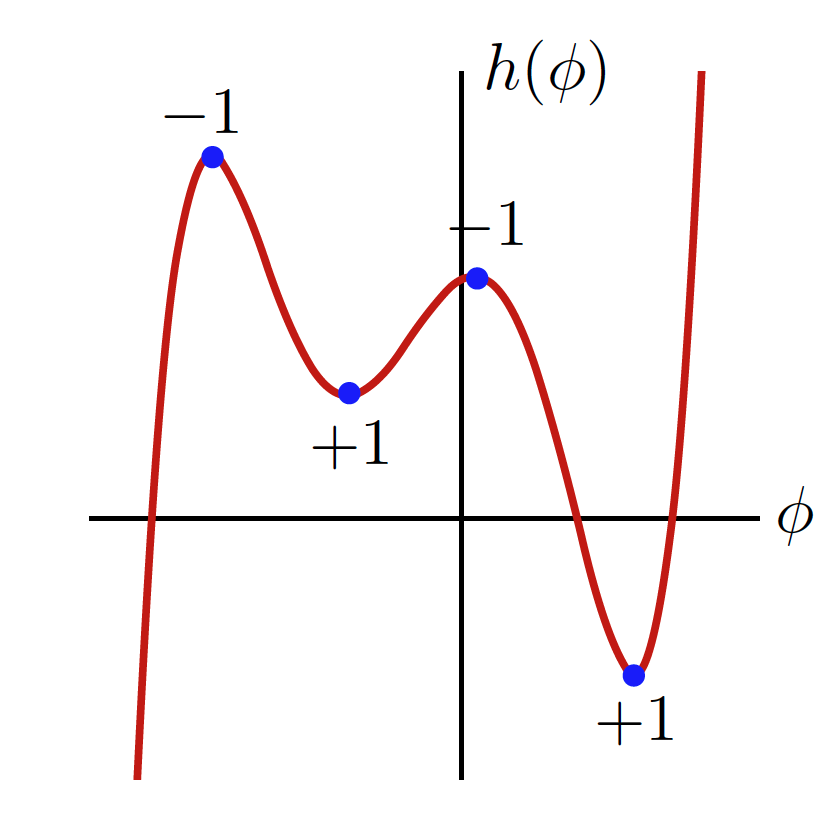
\includegraphics[width=6cm]{../img/Localization.png}
\caption{\textit {The partition function receives contributions just from infinitesimal neighbourhoods of the critical points of $h(\phi)=W(\phi)$. These alternately contribute $\pm1$ accoarding to whether they are minima or maxima}}
\end{figure}

Now we can repeat this argument for expectation value of other operators $\langle O\rangle$ if $QO=O$. this means that also for such expectation values the only contributions are given by a specific set of points, defined by $W'=0$


\end{document}